    \chapter{Introducción al problema}

En este documento se describirá el proceso de confección de una metaheurística basada en un algoritmo genético para encontrar una solución al \textit{Maximum Diversity Problem}.

\section{Definición del problema}
El Maximum Diversity Problem (MDP) Problem consiste en, dado un conjunto de elementos, obtener el subconjunto en el que la diversidad de los elementos sea máxima. Esto es, dado un conjunto $N$ con cardinalidad $|N| = n$, obtener un subconjunto $M \subset N$, con cardinalidad $|M| = m$ y $m < n$ en el que se maximice la diversidad de sus elementos.

La función de diversidad se puede definir tal que:
\begin{equation}
    MD(x) = \sum^{n-1}_{i=0} \sum^{n}_{j=i+1} D_{ij}x_ix_j
\label{max-diversity}
\end{equation}

donde la solución es un número, que determina la diversidad de los elementos elegidos.

$D$ es una matriz de distancias que asocia la distancia de dos elementos del conjunto $N$, de forma que $D_{ij}$ determina la distancia entre el elemento $i$ y el elemento $j$ en el conjunto $N$.

$x$ es una solución posible, que se compone de $n$ elementos donde $x_i \in \{0, 1\}$, es decir, un vector binario. Este vector indica los índices de los elementos del conjunto $N$ que estamos tomando como posible combinación. De esta forma, la cardinalidad de $m$, se calcula como: 

\begin{equation}
    m = \sum_{i=0}^n x_i 
    \label{eq:sum_m}
\end{equation}

lo que nos dice el número de 1 que hay en el vector.

El problema se resume así a calcular qué combinación $x$ ofrece una diversidad mayor. Atendiendo a la ecuación \ref{max-diversity} vemos que el cálculo se sustenta sobre la formación del vector $x$. Al multiplicar $D_{ij}$ por $x_i$ y $x_j$, si alguno de ellos fuera 0, el producto se anula. Solo nos quedamos con aquellos índices en los que ambos sean 1, y el resultado del producto es la distancia entre estos dos elementos (que no necesariamente es conmutativa). Esto nos deja con un vector de distancias cuya suma debemos maximizar.


Como vemos, calcular esto no es una tarea fácil para un número arbitrario de $n$ o de $m$. Para dar un poco de perspectiva, el espacio de soluciones de un ejemplo con $n = 500$ y $m = 50$ es de $2.31 \times 10^{69}$. Se puede observar que el espacio de búsqueda es totalmente inabarcable, siendo este ejemplo uno considerado \textit{mediano}. Puede verse una evolución del crecimiento del espacio de búsqueda en la figura \ref{fig:binom}.

\begin{figure}[h]
    \centering
    
    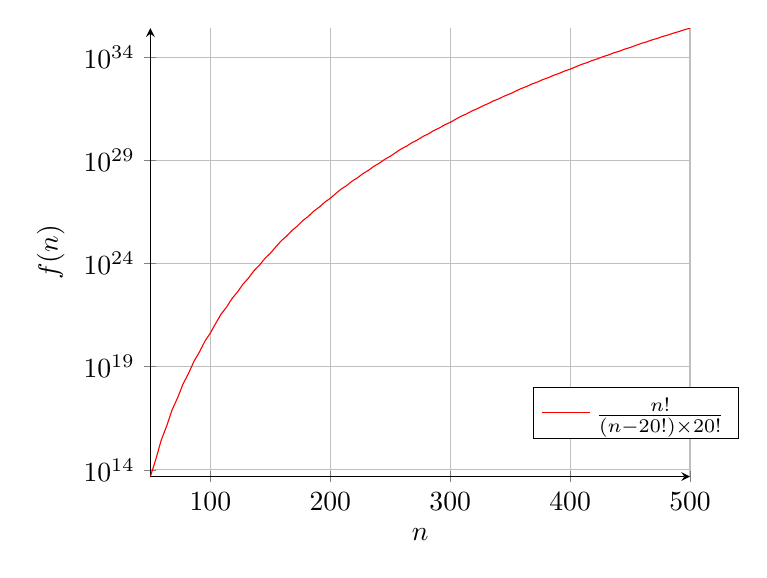
\begin{tikzpicture}
        \centering
        \begin{axis}[
            axis lines = left,
            xlabel = $n$,
            ylabel = {$f(n)$},
            ymode = log,
            grid = major,
            legend style = {at={(0.9,0.2)},
            anchor=north}
        ]
        %Below the red parabola is defined
        \addplot [
            domain=50:500, 
            samples=100, 
            color=red
        ]
        {x! / ((x - 20)! * 20!)};
        \addlegendentry{$\frac{n!}{(n-20!) \times 20!}$}
        
        \end{axis}
        \end{tikzpicture}
    
        \caption{Evolución del crecimiento del espacio de búsqueda en función de $n$, suponiendo que $m = 20$. Vemos que cada línea en el eje $y$ supone un cambio en 5 órdenes de magnitud, lo cual es completamente inabarcable.}
        \label{fig:binom}
    
    \end{figure}


\chapter{Detalles de la implementación}

Describiremos en este capítulo las diferentes consideraciones tomadas de cara a la implementación del algoritmo genético, así como el cálculo de la diversidad de las soluciones.

\section{Consideraciones previas}
Antes de empezar con la descripción de la metaheurística en sí, debemos ser capaces de, dada una potencial solución, calcular su diversidad. Además, debemos ser capaces de cerciorarnos de que dicha solución es válida, es decir, tiene exactamente $m$ unos.

\subsection{Formato de la solución}
Un requisito que presenta nuestro problema es el valor de $m$, que corresponde al número de unos que presenta nuestra solución, o lo que se traduce a exactamente cuál es la mayor diversidad que podemos encontrar en $m$ elementos dada una matriz de distancias $D$.

Para ello, se ha confeccionado una función \jesitt{shape\_solution} que recibe una solución y garantiza que esto es así. Consta de dos bucles \jesitt{while} que preguntan por el número de unos (véase la ecuación \ref{eq:sum_m}), y de no ser el caso correcto, quitan o añaden aleatoriamente para formar correctamente la solución.


\subsection{Cálculo de la biodiversidad}
El cálculo de la biodiversidad es un proceso delicado en el que debemos optimizar al máximo los recursos. Es una operación que se va a ejecutar una enorme cantidad de veces por iteración y es necesario que sea rápida.

Se ha tenido en cuenta que el cálculo está basado en una matriz simétrica, lo que elimina ciertas opciones y puede dar lugar a un resultado más rápido.

El algoritmo luce así:

\begin{enumerate}
    \item En primer lugar calculamos una matriz triangular similar a la nuestra con ceros y unos, y obtenemos los índices donde están los unos. Filtramos el vector resultante quedándonos solo con las parejas de índices en las que el primero sea menor que el segundo.
    \item Dado nuestro vector solución $M$, calculamos todas las posibles combinaciones entre sus genotipos.
    \item Repetimos el proceso anterior, pero con los índices de los genotipos.
    \item Dado el vector con todas las combinaciones de índices de los genotipos, usamos el vector de índices para filtrar el vector de genotipos, quedándonos con las parejas de genotipos en las que el primer índice sea menor que el segundo. Es decir, usamos el vector de índices como máscara.
    \item Esto nos deja con un vector de todas las combinaciones válidas de índices y otro de los genotipos en sí. Los combinamos por columnas.
    \item Teniendo esta estructura de datos, tenemos la información que necesitamos. El cálculo se efectúa iterando por cada elemento de este último vector, multiplicando los dos genes involucrados con el valor que nos devuelva acceder a la matriz con los índices de dichos genotipos, tal y como en la ecuación \ref{max-diversity}.
\end{enumerate}

Este algoritmo hace un uso muy pronunciado de la programación funcional, evitando bucles o condicionales. En principio, se están considerando combinaciones que resultan en 0, ya que uno de los genotipos es 0 en muchos de los casos. Aún así, esto es más rápido que simplemente preguntar con un condicional por solo aquellas combinaciones que tengan un 1 en ambos. Además, utilizando las subrutinas en C de \jesitt{numpy}, esto acelera el proceso. Debemos tener en cuenta, aún así, que python es un lenguaje interpretado y que, necesariamente va a ser más lento que C++, ya que no está pensado para esto.


\subsection{Paralelización del cálculo}
Por último, hablaremos de optimización del rendimiento. Este problema es altamente paralelizable ya que, para cada generación, debemos tener un vector de diversidades que calcular, cada una independientemente, para luego compararlas y efectuar las demás operaciones del algoritmo genético.

Es por ello que hacemos uso de paralelización del cálculo de la biodiversidad para cada solución en cada generación. Suponiendo que la población inicial es de 50 soluciones, paralelizamos el cálculo de la diversidad de cada una de esas soluciones, ya que son complmetamente independientes. Esto reduce el tiempo de cálculo en un 40\% aproximadamente. 


\section{Implementación del algoritmo genético}
En esta sección se discutirán las diferentes consideraciones para la implementación del algoritmo genético.

\section{Topología}

La topología de nuestro algoritmo es muy similar a la que podamos encontrar en cualquier libro, aunque se siguió especialmente la del libro \textit{Introduction to Evolutionary Computing}~\cite{evolutionaryEiben}, y la del \textit{Handbook of Heuristics}~\cite{handbookMart}.


En esencia, generamos un conjunto de soluciones aleatoriamente y calculamos su diversidad. A partir de ahí, empieza el ciclo del algoritmo genético. Tomamos las mejores soluciones, las cruzamos, mutamos y calculamos diversidad, formando la nueva generación. Esta generación formada será la entrada para el siguiente ciclo en el que se repite todo.

Este bucle se repite hasta que se alcance una condición de parada, que puede ser un tiempo límite, un número de iteraciones, etc.

En nuestro caso particular, se utiliza un sistema basado en un contador de iteraciones máximo, así como un contador de \textit{paciencia}. En esencia, si superamos el máximo número de iteraciones provisto, devolvemos la mejor solución encontrada.

Aún así, podremos salir del bucle de otra forma. El contador de paciencia mide cuántas iteraciones llevamos sin obtener una mejor solución global. Si se calcula una generación en la que la mejor solución hasta ahora no mejora, el contador aumenta. Si el contador iguala al valor provisto de paciencia, se asumirá que el algoritmo ha convergido, no necesitando ejecutar todas las iteraciones que resten.

Podemos ver una versión simplificada en el algoritmo \ref{alg:genetic}.

\begin{algorithm}[h]
    G$_{0}$ = GenerateRandomSolutions(maxPopulation)\;
    f$_{0}$ = Evaluate(G$_{0}$)

    $i = 1$\;
    \While{not stopCondition}{
        parents $\gets$ Selection(G$_{i-1}$)\;
        G$_{i}$ $\gets$ Crossover(parents)\;
        f$_{i}$ $\gets$ Evaluate(G$_{i}$)\;

        i $\gets$ i + 1\;
        \eIf{lastBestSolution <= currentBestSolution}{
            patience $\gets$ patience + 1\;
        }
        % else
        {
            patience $\gets$ 0\;
        }

        \If{i == maxIterations or patience == maxPatience}{
            stopCondition $\gets$ True\;}
        }
        \Return BestSolution\;
    
    \caption{Breve resumen de la topología de nuestra versión del algoritmo genético.}
    \label{alg:genetic}
\end{algorithm}

\subsection{\jesitt{Selection}: elección de los mejores}
La selección de los mejores individuos de cada generación se acomete mediante un parámetro \jesitt{k\_top} provisto, que toma las \jesitt{k\_top} mejores soluciones de la generación actual.

\subsection{\jesitt{Crossover}: cruce entre soluciones}
Para el crossover se han definido dos cruces: el cruce clásico y el cruce a dos puntos. Estos cruces están definidos en \cite{handbookMart}, así como en cualquier artículo relacionado con algoritmos genéticos.

\section{Marco de trabajo y equipo utilizado}
En esta sección explicaremos el equipo utilizado y el marco de trabajo de este proyecto, con objeto de que la replicación de la experimentación sea lo más sencilla posible.

\subsection{Equipo utilizado}
Comenzamos con el equipo utilizado. En cuanto a hardware, se dispone de estos equipos:

\begin{itemize}
    \item MacBook Air, i7 11th gen, 4 núcleos con hyperthreading, 8 núcleos en total, 16GB RAM. MacOS 11.3.1, Python 3.9
    \item PC HP con i7 6th gen, 4 núcleos con hyperthreading, 8 núcleos en total, 16 GB RAM. Ubuntu 20.04, Python 3.8
\end{itemize}

En ambos se obtiene un rendimiento similar, aunque la experimentación completa se acometió con el PC HP, que tiene un sistema de ventilación y refrigeración más apropiado que el de cualquier portátil, lo que implica que podrá mantener velocidades de procesador más altas durante más tiempo.

\subsection{Marco de trabajo}
El marco de trabajo se inscribe en la utilización de Python para la implementación. La versión de Python es 3.8-3.9, que, para nuestro caso, pueden considerarse como similares ya que no se hace uso de las diferencias entre las distintas versiones.

Se ha incidido en el uso de \jesitt{numpy} para la implementación, ya que es una interfaz bastante sencilla para subrutinas de C/C++, que son mucho más rápidas que Python puro. Por ello, toda la generación de números aleatorios y la computación de grandes matrices o vectores se ha acometido con \jesitt{numpy}. La semilla utilizada ha sido 7.

\subsection{Instancias utilizadas}
Para la ejecución del algoritmo, se han provisto una serie de 30 archivos con una lista de números, que corresponde a lo que sería la triangular superior de la matriz de distancias de nuestro problema. Estas instancias han sido probadas y se ha experimentado con ellas en otras ocasiones, por lo que podemos comparar los resultados fácilmente para ver cómo lo hace nuestra versión.

\section{Resultados y estadísticas}
Veremos en esta sección una serie de tablas comparativas con el trabajo previamente realizado en estas instancias en relación con los resultados que nosotros hemos obtenido.



